\listfiles
%\documentclass[a4paper, 12pt, pdftex]{scrreprt}
\documentclass[12pt,a4paper,oneside,ngerman,pdftex]{report}
\usepackage[utf8]{inputenc}
\usepackage[T1]{fontenc} % fuer internationale korrekte Silbentrennung
\usepackage{lmodern} % fuer internationale korrekte Silbentrennung
%\usepackage{ae} % Schoene Schriften fuer PDF-Dateien
\usepackage{palatino}
%\usepackage[round]{natbib}
\usepackage[ngerman]{babel}
%\usepackage[ansinew]{inputenc} % ���� lassen sich uncodiert verwenden
\usepackage{graphicx}
\usepackage{svg}
\usepackage{todo}
\usepackage{setspace}
\usepackage{courier}
\usepackage{color}
\usepackage{anysize}
%\usepackage{SIunits} % beisst sich mit amssymb
\usepackage{wrapfig} % Wrapping the text around a figure
\graphicspath{{images/}} % alle Bilder werden im angegebenen Unterverzeichnis gesucht
%\usepackage{epstopdf} % Zur direkten Einbindung von eps-Dateien
%\usepackage{rotating} % Zum einf\"ugen von Bildern in Querformat

%\usepackage{float}	% Option H f\"ur figure wird bereitgestellt
\usepackage{placeins}  % Figures fest positionieren: \FloatBarrier setzt Markierung zum Fortsetzen des Textes
\usepackage{array}	% fuer myBox notwendig
\usepackage{multirow} % Spalten, Zeilen k\"onnen in Tabellen zusammengefasst werden
\usepackage{tabularx} % Gleichmaessige Verteilung der Spalten moeoglich
\usepackage{hhline} % horizontale Doppellinie, aber ohne Unterbrechung der vertikalen Linie
\usepackage{amsmath} % Verbesserter Mathesatz
\allowdisplaybreaks % Erlaubt umbr\"uche in align-Umgebungen
\usepackage{amssymb} % Symbole
\usepackage{paralist} % enumerate oder itemize in compakterer Form
\usepackage{blindtext}
% format=plain ist durch das KOMA-Script verf\"ugbar
\usepackage[format=plain,font=normalsize,labelfont=sf,textfont=it]{caption}
%font=small
%margin=40pt,format=hang,justification=centerlast,singlelinecheck=false,indention=-1cm]{caption}
\usepackage{fancyhdr}
\usepackage{hyperref}
\usepackage{todo}
\usepackage{nameref}

\usepackage{lscape} % ermoeglicht \begin{landscape} fuer querformat
%\usepackage{currfile} % provides the file name and path information of the current input file

\usepackage{multicol}

\usepackage{pdfpages}



%Define the listing package
\usepackage{listings} %code highlighter
\usepackage{color} %use color
\definecolor{mygreen}{rgb}{0,0.6,0}
\definecolor{mygray}{rgb}{0.5,0.5,0.5}
\definecolor{mymauve}{rgb}{0.58,0,0.82}

%Customize a bit the look
\lstset{ %
backgroundcolor=\color{white}, % choose the background color; you must add \usepackage{color} or \usepackage{xcolor}
basicstyle=\footnotesize, % the size of the fonts that are used for the code
breakatwhitespace=false, % sets if automatic breaks should only happen at whitespace
breaklines=true, % sets automatic line breaking
captionpos=b, % sets the caption-position to bottom
commentstyle=\color{mygreen}, % comment style
deletekeywords={...}, % if you want to delete keywords from the given language
escapeinside={\%*}{*)}, % if you want to add LaTeX within your code
extendedchars=true, % lets you use non-ASCII characters; for 8-bits encodings only, does not work with UTF-8
frame=single, % adds a frame around the code
keepspaces=true, % keeps spaces in text, useful for keeping indentation of code (possibly needs columns=flexible)
keywordstyle=\color{blue}, % keyword style
% language=Octave, % the language of the code
morekeywords={*,...}, % if you want to add more keywords to the set
numbers=left, % where to put the line-numbers; possible values are (none, left, right)
numbersep=5pt, % how far the line-numbers are from the code
numberstyle=\tiny\color{mygray}, % the style that is used for the line-numbers
rulecolor=\color{black}, % if not set, the frame-color may be changed on line-breaks within not-black text (e.g. comments (green here))
showspaces=false, % show spaces everywhere adding particular underscores; it overrides 'showstringspaces'
showstringspaces=false, % underline spaces within strings only
showtabs=false, % show tabs within strings adding particular underscores
stepnumber=1, % the step between two line-numbers. If it's 1, each line will be numbered
stringstyle=\color{mymauve}, % string literal style
tabsize=2, % sets default tabsize to 2 spaces
title=\lstname % show the filename of files included with \lstinputlisting; also try caption instead of title
}
%END of listing package%

\definecolor{darkgray}{rgb}{.4,.4,.4}
\definecolor{purple}{rgb}{0.65, 0.12, 0.82}

%define Javascript language
\lstdefinelanguage{JavaScript}{
keywords={typeof, new, true, false, catch, function, return, null, catch, switch, var, if, in, while, do, else, case, break},
keywordstyle=\color{blue}\bfseries,
ndkeywords={class, export, boolean, throw, implements, import, this},
ndkeywordstyle=\color{darkgray}\bfseries,
identifierstyle=\color{black},
sensitive=false,
comment=[l]{//},
morecomment=[s]{/*}{*/},
commentstyle=\color{purple}\ttfamily,
stringstyle=\color{red}\ttfamily,
morestring=[b]',
morestring=[b]"
}

\lstset{
language=JavaScript,
extendedchars=true,
basicstyle=\footnotesize\ttfamily,
showstringspaces=false,
showspaces=false,
numbers=left,
numberstyle=\footnotesize,
numbersep=9pt,
tabsize=2,
breaklines=true,
showtabs=false,
captionpos=b
}




\setlength{\parindent}{0pt}
\setlength{\headheight }{15pt}

\usepackage{datetime} % zur Definition von \pdfdate

\pdfinfo{
	/Title (Bachelorarbeit)
	/Subject ()
	/Author (Johannes Schmitt)
  /CreationDate ()
  /ModDate ()
}
\sffamily	

% #############################################################
\usepackage{amsthm} % Definitionen, theorems
% #############################################################
\newtheoremstyle{myDefinition}   
  {24pt}   %Space above    
  {10pt}   %Space below
  {\itshape} % \itshape        %Body font: original {\normalfont}    
  {}        %Indent amount (empty = no indent,%\parindent = paraindent)    
  {\normalfont}  %Thm head font original    \normalfont\bfseries 
  {}        %Punctuation after theorem head
  { }        %Space after theorem head
  {\sffamily\bfseries {\thmname{#1}\thmnumber{ #2}\thmnote{ (#3)}} } %\normalfont\bfseries} % Theorem head spec
\theoremstyle{myDefinition}
\newtheorem{Def}{Definition}[chapter]

\newtheoremstyle{mySatz}   
  {24pt}   %Space above    
  {10pt}   %Space below
  {\itshape} % \itshape        %Body font: original {\normalfont}    
  {}        %Indent amount (empty = no indent,%\parindent = paraindent)    
  {\normalfont}  %Thm head font original    \normalfont\bfseries 
  {}        %Punctuation after theorem head
  { }        %Space after theorem head
  {\sffamily\bfseries {\thmname{#1}\thmnumber{ #2}\thmnote{ (#3)}} } %\normalfont\bfseries} % Theorem head spec
\theoremstyle{mySatz}
\newtheorem{satz}{Satz}[chapter] 

% #############################################################


\begin{document}
% !TeX root = BA_Gliederung.tex

\begin{titlepage}



% Title
\begin{flushright}
\huge \bfseries {Bachelorarbeit}\\[1.4cm]
\huge \bfseries {Konzeption und Implementierung einer cross-Plattform Smartphone App}\\[0.4cm]
%\\large \bfseries {}\\[4cm]
\end{flushright}

\begin{flushright}
	\textsc{Johannes Schmitt}\\
\end{flushright}


\vfill % Bottom of the page

\renewcommand{\arraystretch}{1.5}
\begin{flushleft}
	\begin{tabular}[H]{ll}
    \large{Letzte \"Anderung:} & \large{\today} \\
	\end{tabular}
\end{flushleft}

\renewcommand{\arraystretch}{1}

\vspace{24pt}


\end{titlepage}

	\pagestyle{plain}	%Default-Einstellung; Leere Kopfzeile und eine Fu�zeile bestehend aus der zentrierten Seitenzahl
	\pagestyle{headings} %In Kopfzeile: Seitenzahl, �berschrift-Informationen; die Fu�zeile bleibt leer. 
	\pagenumbering{roman}
	\setcounter{page}{1}
	
  \setcounter{secnumdepth}{3} % Numerierung auch für \subsubsection
	\setcounter{tocdepth}{1}  % nimmt nur Sections auf, fuer mehr Tiefe eine hoehere Zahl waehlen
	 \tableofcontents   % Inhaltsverzeichnis
	 \todo{Bildunterschriften Halbsätze}
	\listoffigures     % Abbildungsverzeichnis
	\lstlistoflistings % Listingsverzeichnis
	
\pagestyle{fancy}
	\lhead{\slshape \ifthenelse{\equal{\rightmark}{}}{\leftmark}{\rightmark}}
	\rhead{\thepage} %Kopfzeile links
	\lfoot{} %{\footnotesize }}
	\cfoot{}
	\rfoot{} %{\footnotesize Seite \thepage}}

	\pagenumbering{arabic}
	\setcounter{page}{1}
	\onehalfspacing

	
	% !TeX root = Bachelorarbeit.tex
\chapter{Einleitung}
\label{Einleitung}

\section{Motivation}
\emph{Bustracker} ist eine Fallstudie im Projekt \glqq Digitale Kommune\grqq{} der Entwicklungsagentur Rheinland-Pfalz e.V. \emph{Bustracker} soll die Möglichkeit demonstrieren in ländlichen Gebieten den Schulweg der eigenen Kinder zu beobachten. 

In vielen Gemeinden müssen Schüler oder sogar Kindergartenkinder über weite Strecken mit dem Bus zu ihrer Betreuung oder Lerninstitution fahren. In den seltensten Fällen sind noch Betreuungspersonen im Bus vorhanden. Die gängige Praxis, die Kinder durch Eltern mit dem \gls{gls:kfz} an die Schule/den Kindergarten zu bringen, führt zunehmend zu einer Verkehrsüberlastung in den Bereichen um die Betreuungs- bzw. Lernstätte. Die Eltern versuchen, teilweise unter Ignoranz der Straßenverkehrsordnung, den Weg zum Bus oder zur Schule zu verkürzen. 
Damit geht eine erhöhte Gefahr für die Kinder einher, was die Eltern eigentlich durch den Transport per \gls{gls:kfz} zu vermeiden versuchen. 

\emph{Bustracker} soll Eltern die Möglichkeit geben ihre Kinder guten Gewissens mit dem Bus fahren zu lassen.
Plötzlich auftretende Ereignisse, wie z. B. eine Panne am Bus oder eine Straßensperrung können früher erkannt werden, da die Eltern mit \emph{Bustracker} den Schulweg ihres Kindes verfolgen können. Dadurch kann früher reagiert und eine andere Transportmöglichkeit organisiert werden. Die Eltern wissen jederzeit wo sich ihr Kind befindet.  

\emph{Bustracker} implementiert verschiedene Technologien und dient zum Testen und Entwickeln des Konzeptes.


\section{Überblick}
Im Kapitel \textbf{\nameref{Verwendete Technologien}} wird auf die in diesem Projekt verwendeten Softwaretechnologien eingegangen. Die verwendeten Werkzeuge sind ebenfalls in diesem Kapitel beschrieben.

Das Kapitel \textbf{\nameref{Organisation}} beschreibt die Art und Weise wie die Entwicklung organisiert wurde. Der komplette Verlauf ist dort ebenfalls beschrieben.

\textbf{\nameref{Frontend}} erklärt den Aufbau und die Anwendung der in dieser Arbeit entwickelten App.

\textbf{\nameref{Backend}} enthält die Erklärungen und Beschreibungen zu den einzelnen Teilen der Software.

Im Kapitel \textbf{\nameref{Fazit und R\'{e}sum\'{e}}} wird das Projekt kurz zusammengefasst. Vor- und Nachteile sowie gesammelte Erfahrungswerte werden im Kapitel \textbf{\nameref{Lessons learned}} besprochen. In diesem Kapitel werden ebenfalls Lösungsstrategien für die während der Entwicklung aufgetretenen Probleme dargestellt. Im Anschluss daran wird im \textbf{\nameref{sec:Ausblick}} weitere Verbesserungsvorschläge oder weitere Modifikationen der App besprochen.

	% !TeX root = Bachelorarbeit.tex
\chapter{Verwendete Technologien}
\label{Verwendete Technologien}
\emph{Bustracker} ist in Form einer Client-Server Architektur realisiert.  Die Idee Positionsdaten über mehrere Geräte zu verteilen macht es erforderlich diese Daten zentral zu halten. Bei \emph{Bustracker} kommt ein Datenbankserver zum Einsatz. Dieser nimmt die Positionsdaten der Clients im Tracking-Modus entgegen und liefert die Daten an die Clients im Watch-Modus. Als Clients werden die Endgeräte der Nutzer bezeichnet. Die Clients kommunizieren per \nameref{REST} - \nameref{API} (\gls{gls:rest} \gls{gls:API}) mit der Datenbank. In Abbildung \ref{fig:CSArchitektur} ist die Struktur dargestellt. 

\begin{figure}[htbp] 
	\centering
	\includegraphics[width=0.8\textwidth]{images/CSArchitektur.png} 
	\caption{Äußere Architektur von \emph{Bustracker}}
	\label{fig:CSArchitektur}
\end{figure}

Die Architektur der App \emph{Bustracker} selbst ist in Abbildung \ref{fig:innereArchitektur} dargestellt. Die App ist eine \glqq Single Page Application\grqq{}. Der interaktive Teil ist als \gls{gls:html}-Komponente mittels <ion-app> - Tag eingebunden. An dieser Stelle wird das \glqq Root-Element\grqq der Komponente geladen. Die Komponente besteht aus \emph{Declarations}, also den Seiten und den \emph{Providers}, diese enthalten die Programmlogik.

\begin{figure}[htbp] 
	\centering
	\includegraphics[width=0.8\textwidth]{images/AppArchitektur.png} 
	\caption{Innere Architektur von \emph{Bustracker}}
	\label{fig:innereArchitektur}
\end{figure}

Um \emph{Bustracker} auf verschiedenen Platformen einsetzen zu können, muss es vermieden werden, native Funktionen bestimmter Geräte oder Betriebsysteme direkt zu verwenden. Für diesen Prototypen wurde \nameref{sec:Angular}, ein Framework zur Erstellung von Single Page Applications, eingesetzt. Um die nativen Gerätefunktionen, wie z. B. \gls{gls:gps} oder Bluetooth in \emph{Bustracker} zu nutzen wird \nameref{sec:Cordova} verwendet. 
Bei der Entwicklung kommt \nameref{ionic} als übergeordnetes Framework zum Einsatz. Ionic verwendet verschiedene Befehle und Konzepte von Angular und Cordova bereits implizit. 
Die Entwicklungssprache ist \nameref{typescript}, eine Spracherweiterung von Javascript, mit zusätzlicher Syntax und einer Typisierung.
 

\section{Ionic 4}
\label{ionic}
Die Auswahl des Frameworks begründet sich auf die Antworten folgender Fragen:
\begin{description}
\item[In welchen Sprachen ist der/die Entwickler erfahren?] \hfill \\
Der Entwickler hat Erfahrung in Java und TypeScript. 

\item[Ist es eine native Anwendung oder ist sie webbasiert?] \hfill \\
Die Anwendung soll platformübergreifend funktionieren und die nativen Funktionen des jeweiligen Endgeräts unterstützen. Die Anwendung ist grundsätzlich webbasiert, jedoch ist dies für den Nutzer nicht offensichtlich.

\item[Welche Funktionalitäten werden benötigt und sind diese abgedeckt?] \hfill \\
Die benötigten Funktionen sind \gls{gls:gps}, Bluetooth, iBeacon, Festspeicher und \newline HTTP"~Kommunikation (\gls{gls:http}). Die Funktionen sind über die \emph{native Plugins} abgedeckt.

\item[Werden GUI-Elemente geboten?] \hfill \\
Ionic bietet eine Vielzahl von GUI-Elementen für iOS und Material Design. Diese umfassen vor Allem Interaktions- und Anzeigeelemente. \cite{ionicGUI}

\item[Sind Schnittstellen zu z. B. Datenbanken vorhanden ?] \hfill \\
Verschiedene Schnittstellen können via Plugin nachinstalliert werden.

\item[Ist das Framework zukunftsfähig?] \hfill \\
Ja, das Ionic-Framework wird kontinuierlich weiterentwickelt. Dies lässt sich hervorragend am sogenannten \glqq Pulse\grqq des \emph{Ionic}-Repositories ablesen. \cite{IonicPulses}

\item[Entstehen Kosten für das Framework?] \hfil \\
Ionic unterliegt der sogenannten MIT-Lizenz \cite{mitlizenz} und darf privat sowie kommerziell kostenlos verwendet werden.
\end{description}


Basierend auf den Antworten, wurde das Ionic-Framework ausgewählt. In einem vorangegangenen Praxisprojekt \cite{PraxBerJoSc} wurde Ionic bereits erfolgreich verwendet.


Ionic 4 ist ein frei verfügbares Open-Source SDK zur Entwicklung von nativen und progressiven Web-Apps.
Der besondere Fokus des Frameworks liegt auf mobilen Endgeräten. So kann eine Anwendung gleichzeitig für iOS-, Android- und Windows Phone Geräte entwickelt werden.
Entwickelt werden die Apps auf Basis von \gls{gls:html} 5, \gls{gls:css} 3, Angular 5 und TypeScript. Um auf den einzelnen Geräten die integrierten Hardwarefunktionen nutzen zu können wird Apache-Cordova verwendet. Ionic-Native, ein TypeScript Wrapper für Cordova Plugins wird verwendet, um native Funktionen einfach in die Applikation einzubinden.

Das Ionic Framework steht unter der MIT-Lizenz \cite{mitlizenz}, wodurch es sowohl privat als auch geschäftlich kostenlos verwendet werden kann.

\section{Angular 5}
\label{sec:Angular}
Angular ist ein Web-Framework zur Erstellung von Single-Page Applications (SPA). Es basiert auf TypeScript. Angular verwendet das MVVM-Pattern (Model-View ViewModel). 
Die Komponente (Component) entspricht hier dem ViewModel, welches die UI-Logik enthält. Sie tauscht Daten mit dem Model aus und stellt Methoden und Dienste bereit. 
Die View wird durch Databinding an das ViewModel gebunden und ist somit einfach austauschbar. 
Sie wird unter Verwendung von \gls{gls:html} 5 und \gls{gls:css} 3 erzeugt. 
Das Model enthält alle Inhalte, die durch den Benutzer angezeigt und verändert werden können.
Angular ist seit November 2017 in der Version 5 erhältlich. Das Framework ist Open-Source und Google ist an der Entwicklung beteiligt. Unit-Tests und End-to-End Tests werden von Angular unterstützt.  \cite{angulario}
 

\section{TypeScript}
\label{typescript}
TypeScript ist eine freie Open-Source Programmiersprache, die von Microsoft entwickelt
wird \cite{TSDoc}.  Bei der Programmiersprache handelt es sich um eine typisierte Obermenge von JavaScript.
Sie basiert auf den \gls{gls:ecma} 6 Standard und erweitert die JavaScript Sprache mit einer statischen Typisierung, wie in der Abbildung \ref{img:typescript} zu sehen ist. Um die Kompatibilität zu gewährleisten, ist JavaScript Code gültiger Typescript Code. Ein Browser muss mindestens \gls{gls:ecma} 5 Fähigkeiten haben, damit Typescript ausführbar ist. 
\begin{figure}[htbp]
	\centering
	\includegraphics[scale=0.5]{TypeScript.jpg}
	\caption{TypeScript Sprach-Hierachie \cite{tshirachie}}
	\label{img:typescript}
\end{figure} 

%\begin{figure}[htbp] 
 % \centering
 %    \includegraphics[width=0.8\textwidth]{images/idestypescript.png} 
%  \caption{Empfohlene IDEs für TypeScript}
 % \label{fig:IDEs}
% \end{figure}

\section{Cordova}
\label{sec:Cordova}
Apache Cordova ist ein Open Source Framework zur Entwicklung für mobile Plattformen. Mit Cordova ist es möglich moderne Web-Technologien, wie \gls{gls:html} 5, \gls{gls:css} 3 und JavaScript (hier TypeScript) für plattformübergreifende Entwicklung zu nutzen. Um auf die Sensoren und Daten der einzelnen Geräte zuzugreifen werden Standard APIs der einzelnen Betriebssysteme verwendet. Cordova dient als Mittelschicht zwischen Anwendung und Gerät \cite{cordovaDoku}. Abbildung \ref{img:cordova} zeigt den allgemeinen Aufbau der Architektur.
\begin{figure}[htbp]
	\centering
	\includegraphics[width=0.6\textwidth]{cordova.png}
	\caption{Architektur von Cordova \cite{cordovaDoku}}
	\label{img:cordova}
\end{figure}

\section{iBeacon}
Sogenannte iBeacons sind Bluetooth Low Energy Sender, die nach einem proprietärem von Apple spezifizierten Protokoll, dem iBeacon Protokoll \cite{iBeaconSpec}, arbeiten. Die Idee hinter der Entwicklung der iBeacons war die Durchführung von Lokalisation innerhalb von Gebäuden. Beacons eignen sich aber auch für den Gebrauch im Freien, damit können unabhängig des \gls{gls:gps}-Signals Ereignisse, wie das Erreichen oder Verlassen eines bestimmten Bereichs detektiert werden. Abbildung \ref{img:ibeacon} zeigt eine schematische Darstellung der Technologie.
Zur Identifizierung eines einzelnen Beacons werden bei \emph{Bustracker} vier Parameter verwendet, die nachfolgend erläutert werden:

\begin{description}
\item[UUID] \hfill \\
Die \gls{gls:UUID} gibt in diesem Falle die sogenannte Region an. Eine Beacon Region ist keine Region im Sinne von einem durch geografische 
Merkmale begrenztem Bereich. Sie wird durch die Parameter \gls{gls:UUID}, Major und Minor charakterisiert. So wie ein einzelnes Beacon durch die gleichen Parameter gekennzeichnet ist. Die physische Repräsentation einer Beacon Region ist die Reichweite aller dieser Region zugeordneten Beacons. 
Mehrere iBeacons können die gleiche \gls{gls:UUID} haben. 
Alle Beacons mit der gleichen \gls{gls:UUID} gehören zur gleichen Region. \cite{beaconRegion}

Zum Beispiel könnten 100 Beacons mit der gleichen 
\gls{gls:UUID} einem Busunternehmen zugeordnet sein.
\item[Major] \hfill \\
Der Major-Parameter unterteilt die Beacons einer \gls{gls:UUID}. Zum Beispiel könnte dies eine Linie (Strecke) des Busunternehmens sein.
\item[Minor] \hfill \\
Der Minor-Parameter unterteilt eine Major-Gruppe in einzelne Beacons. Dies könnte einer Haltestelle auf einer Linie entsprechen.
\item[Identifier]\hfill \\
Identifier ist ein String um ein Beacon zu beschreiben. Zum Beispiel könnte das hier der Name der Haltestelle sein.
\end{description}

\begin{figure}[htbp]
	\centering
	\includegraphics[scale=0.7]{images/iBeacon_schema.png}
	\caption{Schematische Darstellung der iBeacon-Technologie}
	\label{img:ibeacon}
\end{figure} 

Zur konkreten Anwendung kommt diese Technologie im \nameref{srv:iBeaconService}. 

\section{REST}
\label{REST}

\gls{gls:rest} bedeutet Representational State Transfer und beschreibt eine Architektur. Eine \gls{gls:rest} \gls{gls:API} ist \textbf{statuslos}, d. h. es gibt keine Nutzersessions. Jede Anfrage erzeugt eine neue Ressource, alle Daten werden nochmals
generiert. Jede dieser Ressourcen ist über eine spezifische URI adressierbar. Ressourcen können in unterschiedlichen Repräsentationen vorliegen. Die gleiche Information kann in unterschiedlichen Formaten abgerufen werden,
z. B. \gls{gls:html} und \gls{gls:json}. 
\cite{Abts2015}

\section{Werkzeuge}

\subsection{WebStorm}
Aus einem vorhergehenden Projekt war die integrierte Entwicklungsumgebung WebStorm bereits bekannt. 
 
In WebStorm sind die Technologien \gls{gls:html}5, TypeScript, Angular und Cordova bereits integriert. Die \gls{gls:IDE} lässt sich durch ein breites Angebot an Plugins erweitern. Webstorm basiert auf der IntelliJ IDEA Plattform und verwendet Konzepte, die bereits durch \glspl{gls:IDE} wie AndroidStudio bekannt sind. 
WebStorm ist auf JavaScript spezialisiert und bietet darauf zugeschnittene Funktionen wie z. B. Codevervollständigung, automatisches Importieren, Signaturinformationen bei Funktionsaufruf und kontextbezogene Hervorhebung von Syntax. Die Integration von Git/Github erwies sich ebenfalls als sehr hilfreich. Es wird kein weiteres Programm neben der \gls{gls:IDE} benötigt.
Das Interface ist in Abbildung \ref{fig:WebStorm} zu sehen.
 
  \begin{figure}[htbp] 
  \centering
     \includegraphics[width=0.9\textwidth]{images/webstorm_weiss.png} 
  \caption{Interface der WebStorm IDE}
  \label{fig:WebStorm}
\end{figure}

\subsection{compodoc}
\label{compodoc}

Um die Verständlichkeit und die Wartbarkeit von Software zu gewährleisten muss eine Dokumentation zum Programmcode existieren. Ein großer Teil der Dokumentation besteht aus Quellcodedokumentation. Der Dokumentationsprozess ist in der Regel aufwendig und bedeutet für die Entwickler zusätzliche Arbeit. Dies führt häufig zu einer lückenhaften und unvollständigen Dokumentation der Software. Um dem vorzubeugen gibt es Tools, die diesen Prozess vereinfachen. 
\textbf{Compodoc} ist ein solches Tool.

Compodoc ist kommandozeilenbasiert und erzeugt eine statische codebasierte Quellcodedokumentation von Angularanwendungen. Die Codedokumentation ist in der Struktur einer Website ausgeführt, sie umfasst eine aufbereitete Ansicht der vom Entwickler im Code eingefügten Kommentare, so dass diese nicht mehrmals geschrieben werden müssen. 
Es besteht die Auswahl zwischen verschiedenen Themes bzw. Templates. Die Templates sind bereits responsiv und unterstützen moderne Webtechnologien.

Diese \glqq Website\grqq{}  wird lokal gehostet und benötigt somit keinen externen Server. Eine mächtige Such-Engine namens \glqq lunr.js\grqq{} sorgt dafür, dass die Dokumentation effizient durchsucht werden kann. Compodoc parsed den Code lediglich, es ist keine TypeScript-Kompilierung notwendig. Durch das Parsen enthält die Dokumentation alle Elemente der Anwendung automatisch. Sie sind im Inhaltsverzeichnis gelistet. Es besteht die Möglichkeit zu jeder Komponente den Quellcode direkt einzusehen. Kommentare die im JSDoc-Format \cite{JSdoc} vorliegen, werden von Compodoc \glqq verstanden\grqq{} und in die Codedokumentation mit aufgenommen. Zur Zeit kann Compodoc \glqq @param, @returns, @link und @example\grqq verarbeiten. Abbildung \ref{fig:JSDemo} zeigt den Quellcode und das Compodoc Ergebnis.

\begin{figure}[htbp] 
	\centering
	\includegraphics[width=0.9\textwidth]{images/composource.png} 
	\includegraphics[width=0.9\textwidth]{images/compoergebnis.png}
	\caption{TypeScript Quellcode und Compodoc Seite im Vergleich.}
	\label{fig:JSDemo}
\end{figure}

	% !TeX root = Bachelorarbeit.tex
\chapter{Organisation}
\label{Organisation}
\section{Workflow}
Der bereits im Praxisprojekt \cite{PraxBerJoSc} etablierte Workflow wurde zu einem großen Teil übernommen. 
Tägliche Treffen jedoch entfielen, da der Autor nicht in einem Team arbeitete.

Anforderungen an die Software wurden als Stories in dem \glqq Issues \grqq-Tab des verwendeten GitHub Repositories als User Story eingetragen. Abbildung  \ref{fig:EinzelStory} zeigt eine solche Story.


\begin{figure}[htbp] 
  \centering
     \includegraphics[width=0.8\textwidth]{images/EinzelStory.png} 
  \caption{Einzelne Story im Issues-Tab des \emph{Bustracker} Repository}
  \label{fig:EinzelStory}
\end{figure}

Es wurden Stories aus dem in Abbildung \ref{fig:IssuesTab} gezeigten IssusesTab gewählt. Nach Abschluss einer Story bzw. Implementierung eines Features, wurde diese mit dem Label \glqq Done\grqq{} versehen. Nach positiver Abnahme wurde die Story dann auf \glqq closed\grqq{} gesetzt und somit geschlossen.

\begin{figure}[htbp] 
  \centering
     \includegraphics[width=0.8\textwidth]{images/issues_tab.png} 
  \caption{Issues-Tab des Repository}
  \label{fig:IssuesTab}
\end{figure}

Um die Positionsdaten zu erfassen und im Anschluß wieder zu verteilen wird eine Datenbank benötigt. Die gewählte Datenbank ist eine sogenannte MariaDB \cite{MariaDBDoku}.
Die gewählte Datenbankstruktur und die benötigten Daten sind in Abb. \ref{fig:ERD} dargestellt.

\begin{figure}[htbp] 
	\centering
	\includegraphics[width=0.8\textwidth]{images/ERDiagramm_bustracker.png} 
	\caption{ER-Diagramm der Bustracker Datenbank}
	\label{fig:ERD}
\end{figure}

 Die API-Entwicklung wurde extern durchgeführt. Die entstandene REST-API ist in \cite{btapidoku} beschrieben. 
\section{Ablauf}

Zu Beginn der Arbeit wurden die benötigten Funktionalitäten für \emph{Bustracker} identifiziert. Diese wären zum einen die Möglichkeiten zur Positionsbestimmung \gls{gls:css} und iBeacons und zum anderen die Anzeige der zuvor bestimmten Position. Dies wurde mittels der Brainstorming Technik durchgeführt. (Abbildung \ref{fig:Brainstorming}).

Für den Prototypen kommt hier aufgrund der einfachen Implementierung und umfangreicher \glspl{gls:API}  GoogleMaps in Frage. Um den Zustand der App speichern zu können bot sich der Zugriff auf den Festspeicher des jeweiligen Endgerätes an.  Um dem eigentlichen Zweck, die Mitteilung der eigenen Position an ein anderes Endgerät zu übertragen, zu entsprechen, müssen die Daten weitergeleitet werden.  Dazu wird bei \emph{Bustracker} eine \nameref{REST} - \nameref{API} eingesetzt.  

\begin{figure}[htbp] 
  \centering
     \includegraphics[width=0.8\textwidth]{images/brainstorming.png} 
  \caption{Ergebnis des Brainstormings}
  \label{fig:Brainstorming}
\end{figure}

\nameref{ionic} bietet eine Reihe von Plugins an, mit denen die native Hardware des Gerätes plattformunabhängig angesprochen wird. Alle Funktionen können mittels solcher \emph{native Plugins} abgebildet werden. Zur konkreten Implementierung siehe Kapitel \nameref{Backend}.

Im Anschluss an diesen Teil erfolgte die Implementierung von Teilfunktionen um mehr über das Verhalten der einzelnen Plugins herauszufinden. Parallel wurde das Aussehen des \gls{gls:gui} in sogenannten Scribbles skizziert. Ein Beispiel ist das Scribble der WatchPage in Abbildung \ref{fig:scribble}. 

\begin{figure}[htbp] 
  \centering
     \includegraphics[width=0.6\textwidth]{images/scribble.png} 
  \caption{Scribble der WatchPage}
  \label{fig:scribble}
\end{figure}

Nach dem Vorbild der Scribbles wurden die Seiten gestaltet. Im Anschluss daran wurden die Komponenten ausgewählt, um die geplanten Funktionalitäten bereitzustellen. Diese Komponenten wurden eingebunden und damit der gewünschte Funktionsumfang geschaffen. Nachdem die Komponenten erfolgreich getestet wurden, erfolgte die externe Anbindung an die \gls{gls:API}.
Am Ende wurde die Benutzeroberfläche einheitlich gestaltet.


	% !TeX root = Bachelorarbeit.tex
\chapter{Frontend}
\label{Frontend}

\section{Aufbau}

\begin{figure}[htbp] 
  \centering
     \includegraphics[width=0.7\textwidth]{images/FlowChart_Bustracker.png} 
  \caption{Ablaufdiagramm \emph{Bustracker}}
  \label{fig:Ablaufdiagramm}
\end{figure}


Die App gliedert sich in folgende Bereiche:
\begin{description}
\item[Watch Bereich] \hfill \\
Im Watch Bereich lädt die App regelmäßig Daten des zu beobachtenden Nutzers von einem Server. 
\item[Track Bereich] \hfill \\
Im Track Bereich führt die App regelmäßig Positionsbestimmungen durch und wartet auf das Entdecken bestimmter iBeacons durch das Gerät. So erkennt die App Checkpoints, in der Regel Haltestellen oder Ziele. 
\item[Konfiguration] \hfill \\
In der Konfiguration wird festgelegt, welcher Nutzer beobachtet wird. In Zukunft wird diese Konfiguration komplexer und umfangreicher werden.
\end{description}


\section{Funktionsweise}

Bei erstmaligem Start werden die sogenannten Permissions abgefragt. Der Nutzer muss der App den Zugriff auf Festspeicher, Bluetooth und \gls{gls:gps} gestatten. Dann gelangt der Nutzer auf die \nameref{HomePage}. Hier wählt der Nutzer aus, ob er seinen Standort mitteilen oder ein anderes Gerät verfolgen möchte. Nur von der Homepage kommt der Nutzer auf die \nameref{ConfigurationPage}. Dort stellt der Nutzer seine eigene ID (die UserID), sowie die ID des zu beobachtenden Geräts (trackingID) ein, anschließend kehrt er auf die \nameref{HomePage} zurück. Abbildung \ref{fig:Ablaufdiagramm} zeigt die App in Form eines Ablaufdiagramms. 



\subsection{API}
\label{API}
Das Akronym \gls{gls:API} steht für \emph{Application Programming Interface} und bedeutet Programmierschnittstelle. Sie definiert in welcher Form Daten, in diesem Fall serverseitig, angenommen und bereitgestellt werden. Sie stellt definierte Funktionen für den Datentransfer bereit. Ein großer Vorteil einer \gls{gls:API} besteht darin, dass sich die interne Datenverwaltung der \gls{gls:API} ändern kann, ohne die Schnittstelle zu beeinflussen.
Abbildung \ref{fig:API} zeigt den Kommunikationsablauf mit \emph{Bustracker}.
Die \gls{gls:API} ist nicht an die jeweilige Anwendung gebunden. Weitere Anwendungen könnten die \gls{gls:API} verwenden, um Daten bereitzustellen oder abzurufen. So wäre es denkbar, Skills für Sprachassistenten zu entwickeln, die auf die \gls{gls:API} Daten zurückgreifen. 

\begin{figure}[htbp] 
  \centering
     \includegraphics[width=0.7\textwidth]{images/APIsequence.png} 
  \caption{\emph{Bustracker} API Sequenzdiagramm}
  \label{fig:API}
\end{figure}

\emph{Bustracker} kommuniziert mit einer \gls{gls:rest} - \gls{gls:API} (siehe Kapitel \ref{REST}), dies ist eine gängige Form für \glspl{gls:API}. Zum Zeitpunkt der Entwicklung befand sich der Server innerhalb des hochschulinternen Netzwerks und war von außen nur per \gls{gls:VPN} zu erreichen. In einer Produktivumgebung wird der Server direkt erreichbar sein, dann mit einer Nutzerauthentifizierung.

\subsection{Speicherstruktur}
\begin{figure}[htbp] 
  \centering
     \includegraphics[width=0.7\textwidth]{images/Speicherstruktur.png} 
  \caption{\emph{Bustracker} Speicherstruktur mit Datenflussrichtung}
  \label{fig:Speicherstruktur}
\end{figure}

Die Struktur des Speichers (siehe Abb. \ref{fig:Speicherstruktur}) wurde so gewählt, dass der \nameref{srv:PersistenzService} keine anderen Injectables instantiiert. 
Der \nameref{srv:LoadService} und der \nameref{srv:SaveService} instantiieren den PersistenzService, der den Festspeicher des Geräts verwaltet. Load- und SaveService werden nur vom \nameref{srv:RTMService} instantiiert. Daraus ergibt sich eine Struktur, die unanfällig für Zirkelbezüge ist.   
Um einen Zirkelbezug, wie in Kapitel 6 aus dem Praxisbericht \cite{PraxBerJoSc} dargestellt zu vermeiden, wurde die Speicherstruktur direkt so ausgestaltet, dass sich keine Injectables gegenseitig instantiieren.
 


	% !TeX root = Bachelorarbeit.tex
\chapter{Backend}
\label{Backend}

\section{HomePage}
\label{HomePage}
Die Homepage erscheint zum Start von \emph{Bustracker}, auf dieser Seite wird die Funktion gewählt. Je nach Auswahl wird die entsprechende Page der App geladen.
\subsection{HTML}
Die \gls{gls:html}-Seite in Abb. \ref{fig:Screens} zeigt zwei Buttons, der obere dient dazu das Tracking zu aktivieren und führt auf die \nameref{pag:TrackingPage}. 
Der untere Button dient dazu, ein anderes Gerät zu verfolgen und führt auf die \nameref{pag:WatchPage}.
Am oberen rechten Rand befindet sich ein \glqq Zahnrad\grqq, bei einem Klick darauf erscheint die \nameref{ConfigurationPage}.
\subsection{CSS}

\begin{lstlisting}[float, language=HTML5, caption=Stylesheet für die Homepage , label=lst:HomeCSS]
page-home {
  .scroll-content {
    background-color: #1C4AFF;
  }
  .toolbar-background {
    background-color: #0D47A1;
  }
  .toolbar-title {
    color: white;
  }
  .icon-only {
    background-color: #0D47A1;
  }
  .icon{
      color:white;
    }
  .icon-only{
    background-color: #0D47A1;
    color: #0D47A1;
    }
  .bar-buttons{
    background-color: #0D47A1;
    color: #0D47A1;
  }
}

\end{lstlisting}

Listing \ref{lst:HomeCSS} zeigt das Stylesheet für die Homepage. Die Anweisungen dienen dazu, den Seitenheader in dunkelblau (Hex: 0D47A1) und die Schrift Weiß (Hex: FFFFFF) zu färben.  Der Seitenhintergrund wird mittels der Zeilen 3 - 5 in einem helleren Blau dargestellt (Hex: 1C4AFF).

\subsection{TypeScript}

Die TypeScript Datei \textbf{home.ts} enthält diejenigen Methoden, die nach Betätigen des jeweiligen Buttons die neue Seite aufrufen. Diese sind im Listing \ref{lst:HomeTypescript} zu sehen.

\begin{lstlisting}[float, language=JavaScript, caption= Methoden zur Navigation , label=lst:HomeTypescript]
 goTracking(){
    this.navCtrl.push(TrackingPage).then(()=> console.log('TrackingPage aufgerufen'));
  }

  goWatch(){
    this.navCtrl.push(WatchPage).then(()=> console.log('WatchPage aufgerufen'));
  }

  goConfig(){
    this.navCtrl.push(ConfigPage).then( ()=> console.log('ConfigPage aufgerufen'));
  }
\end{lstlisting}

\section{ConfigurationPage}
\label{ConfigurationPage}
Die Konfigurationsseite (siehe Abb. \ref{fig:Screens}) bietet die Möglichkeit die eigene NutzerID einzustellen. Weiterhin kann die ID des zu trackenden Nutzers eingestellt werden. 
Die API-Aufrufe erfolgen auf der Tracking Seite mit der eigenen ID. Auf der Watchseite wird die ID des zu trackenden Nutzers verwendet.
\subsection{HTML}
Auf der Configuration Page sind zwei Inputs zu sehen. Der erste ist dazu gedacht, die eigene NutzerID einzugeben. Der zweite Input dient zum Eingeben des zu beobachtenden Nutzers.
Es existiert eine \gls{gls:API} Beschränkung. Die IDs müssen existieren, sonst führt dies zu Fehlern bei der Abfrage.
\begin{lstlisting}[float, language=HTML5, caption= Input mittels Databinding , label=lst:ConfigHTML]
 <ion-item>
    <ion-label color="primary" fixed> Eigene ID</ion-label>
    <ion-input type="number" [(ngModel)]="this.rtm.USER_ID" placeholder="Hier ihre eigene ID"></ion-input>
  </ion-item>
\end{lstlisting}
In Listing \ref{lst:ConfigHTML} ist die dynamische Datenbindung zu sehen. Der Nutzer manipuliert den Input, direkt nach der Manipulation wird der Wert in den \nameref{srv:RTMService} gespeichert. Beim Betreten der Seite wird die jeweilige ID direkt aus dem RTMService geladen. 
\subsection{CSS}
\begin{lstlisting}[float, language=HTML5, caption=Stylesheet für die ConfigurationPage , label=lst:ConfigCSS]
page-konfiguration {

.scroll-content {
background-color: #1C4AFF;
}
.toolbar-background {
background-color: #0D47A1;
}
.toolbar-title {
color: white;
}
.bar-button-default-md, .bar-button-clear-md-default, .bar-button-md-default
{
color: white;
}
}
\end{lstlisting}

Listing \ref{lst:ConfigCSS} zeigt das Stylesheet für die Homepage. Die Anweisungen dienen dazu, den Seitenheader in dunkelblau (Hex: 0D47A1) und die Schrift Weiß (Hex: FFFFFF) zu färben. Die Zeilen 12 - 15 dienen dazu, den \glqq Zurück\grqq{}-Pfeil in Weiß einzufärben. Der Seitenhintergrund wird mittels der Zeilen 3 - 5 in einem helleren Blau dargestellt (Hex: 1C4AFF).

\subsection{TypeScript}

In der TypeScript Datei wird der \nameref{srv:RTMService} im Konstruktor instantiiert um das sogenannte \emph{two-way-databinding} zu ermöglichen.  Siehe Listing \ref{lst:ConfigTypeScript}

\begin{lstlisting}[float, language=JavaScript, caption= Konstruktor ConfigurationPage , label=lst:ConfigTypeScript]
 constructor(public navCtrl: NavController, public navParams: NavParams, private rtm: RTMProvider) {}
\end{lstlisting}

\section{TrackingPage}
\label{pag:TrackingPage}

Die TrackingPage (Abb. \ref{fig:Screens}) zeigt die Eigene Position als LatLong Koordinate und als Adresse an. Zusätzlich wird der letzte Checkpoint angezeigt. Über einen Schalter kann der Nutzer das Tracking aktivieren oder deaktivieren.
\subsection{HTML}

Die \gls{gls:html}-Seite der TrackingPage zeigt oben einen Schalter zum Aktivieren oder Deaktivieren des Trackings. Darunter befindet sich ein Feld mit dem Längen- und Breitengrad, sowie die, sich aus dieser Koordinate ergebende Adresse. Die Daten werden via Databinding aus dem \nameref{srv:RTMService} bezogen. Listing \ref{lst:TrackingHTML}

\begin{lstlisting}[float, language=HTML5, caption= Adresse via Databinding , label=lst:TrackingHTML]
<ion-item>
 {{this.rtm._config.lat}}:Latitude {{this.rtm._config.lng}}:Longitude 
 Strasse: {{this.rtm.address.thoroughfare}} Nr: {{this.rtm.address.subThoroughfare}}
  PLZ: {{this.rtm.address.postalCode}} Ort: {{this.rtm.address.locality}}
</ion-item>
\end{lstlisting}


\subsection{CSS}

\begin{lstlisting}[float, language=HTML5, caption=Stylesheet für die TrackingPage , label=lst:TrackingCSS]
page-tracking {
.scroll-content {
background-color: #1C4AFF;
}
.toolbar-background {
background-color: #0D47A1;
}
.toolbar-title {
color: white;
}
.bar-button-default-md, .bar-button-clear-md-default, .bar-button-md-default
{
color: white;
}
}
\end{lstlisting}

Listing \ref{lst:TrackingCSS} zeigt das Stylesheet für die Homepage. Die Anweisungen dienen dazu, den Seitenheader in dunkelblau (Hex: 0D47A1) und die Schrift Weiß (Hex: FFFFFF) zu färben. Die Zeilen 12 - 15 dienen dazu, den \glqq Zurück\grqq{}-Pfeil in Weiß einzufärben. Der Seitenhintergrund wird mittels der Zeilen 3 - 5 in einem helleren Blau dargestellt (Hex: 1C4AFF).

\subsection{TypeScript}

Die TrackingPage instantiiert den \nameref{srv:RTMService}, den \nameref{srv:TrackerService} und den \nameref{srv:iBeaconService}, um auf Werte zugreifen zu können, sowie Methoden der Dienste zu verwenden.


Nachdem die Seite vollständig geladen ist, wird die Funktion \emph{ionViewDidLoad()} ausgeführt. Innerhalb dieser Funktion wird der Status des \glqq trackingIndicators \grqq abgefragt, basierend darauf wird das Tracking gestartet oder gestoppt. Dazu kommt eine If-Abfrage in Form eines bedingten ternären Operators zum Einsatz \cite{TernärerOperator}.  Siehe Listing \ref{lst:TrackingTypescript}. 

\begin{lstlisting}[float, language=JavaScript, caption= ionViewDidLoad()-Methode der TrackingPage , label=lst:TrackingTypescript]
 ionViewDidLoad() {
    console.log('ionViewDidLoad TrackingPage');
    (this.rtm.trackingIndicator.valueOf()== true) ? this.trackerService.startTracking() : this.trackerService.stopTracking();
    console.log(this.rtm.trackingIndicator.valueOf());
    this.beaconService.initBeacon();
}
\end{lstlisting}

Im Anschluss wird der \nameref{srv:iBeaconService} gestartet. Beim Verlassen der Seite wird automatisch der Inhalt vom \nameref{srv:RTMService} auf den Festspeicher übertragen.

\section{WatchPage}
\label{pag:WatchPage}

Die WatchPage zeigt die Position des beobachteten Geräts auf einer Karte, als LatLong-Koordinate und als Adresse an.

\subsection{HTML}

Die WatchPage (Abb. \ref{fig:Screens}) zeigt eine GoogleMaps-Karte mit Positionsinformationen des zu beobachtenden Nutzers an. Die Karte stellt der \nameref{MapsService} bereit. Sie wird an das \emph{div} mit dem Namen 
\glqq map\_canvas\grqq{} gebunden.
Zusätzlich ist die aktuelle Adresse der Position und der letzte Checkpoint zu sehen.
Adresse und Checkpoint werden hier analog zur \nameref{pag:TrackingPage} vom \nameref{srv:RTMService} zur Verfügung gestellt und angezeigt.

\subsection{CSS}

Die Google Karte benötigt einen transparenten Hintergrund und ein benanntes <div>. Hier wird die Karte in einer sogenannten ion-card angezeigt, einem Template des Ionic-Frameworks. Mittels \gls{gls:css} wird diese Card als transparent gekennzeichnet. Listing \ref{lst:WatchCSS} zeigt die Style-Konfiguration für das <div> und die Klasse \glqq transparent-card\grqq{}. Zusätzlich sind die Stylingoptionen für sichtbare \gls{gls:css}-Elemente eingetragen, analog zu den anderen Seiten um das Erscheinungsbild möglichst einheitlich zu gestalten.

\begin{lstlisting}[float, language=HTML5, caption= Transparentes Canvas und Styling der WatchPage, label=lst:WatchCSS]
page-watch {
  #map_canvas {
    height: 90%;
  }
  .transparent-card{
    background-color: transparent;
  }
  .scroll-content {
  background-color: #1C4AFF;
  }
  .toolbar-background {
  background-color: #0D47A1;
  }
  .toolbar-title {
  color: white;
  }
  .bar-button-default-md, .bar-button-clear-md-default, .bar-button-md-default
  {
  color: white;
  }
}
\end{lstlisting}

\subsection{TypeScript}

Die WatchPage verfügt, analog zur \nameref{pag:TrackingPage}, über eine \emph{ionViewDidLoad()}-Methode. In dieser wird der \nameref{MapsService} initialisiert. 
Die Seite bietet verschiedene Methoden zum Abrufen und Zeichnen der Position des gewünschten Teilnehmers. Listing \ref{lst:WatchTypeScript} zeigt die Methode zum Abrufen der letzten Position eines Teilnehmers.



\begin{lstlisting}[float, language=JavaScript, caption=Methode zum Abruf der letzten Position , label=lst:WatchTypeScript]
getSinglePos(){
  this.apiService.getLastLocationById(this.rtm.trackingID).then(
    (data)=> {
    this.rtm.lat = data.lat;
    this.rtm.long = data.lon;
    this.trackerService.geoCode();
  }).catch((err)=> {console.log('Fehler getSinglePos: ' + JSON.stringify(err))});
}
\end{lstlisting}


\begin{figure}[htbp] 
	\centering
	\includegraphics[width=0.35\textwidth]{images/Homepage.png}
	\includegraphics[width=0.35\textwidth]{images/Configpage.png}
	\caption{Home-  und Configpage von \emph{Bustracker}}
	\label{fig:Screens}
\end{figure}
\begin{figure}[htbp]
	\centering
	\includegraphics[width=0.35\textwidth]{images/Trackingpage.png}
	\includegraphics[width=0.35\textwidth]{images/Watchpage.png}
	\caption{Tracking- und Watchpage von \emph{Bustracker}}
\end{figure}

\pagebreak
\section{APIService}
\label{srv:APIService}
Der \gls{gls:API} Service übernimmt die Kommunikation mit der \gls{gls:rest}-\gls{gls:API} von \emph{Bustracker}. 
\subsection{Verwendete Plugins}
@angular/common/http \cite{AngularHttp}
\subsection{Arbeitsweise}
Der Service stellt eine \textbf{POST} Methode bereit, mit der die Daten des Mobilgeräts  an die API gesendet werden. Diese Funktion kommt beim Tracking \ref{srv:TrackerService} zum Einsatz.
Das Abrufen der Daten geschieht mittels verschiedener \textbf{GET} Methoden. Es können alle gespeicherten oder die letzte gespeicherte Position eines mittels \textbf{ID}{} festgelegten Teilnehmers abgerufen werden. Listing \ref{lst:APIService}.

\begin{lstlisting}[float, language=JavaScript, caption= Rückgabe aller gültigen Positionsdaten der jeweiligen TrackingID , label=lst:APIService]
getAllDataById(id: number) {
    console.log('GET URL: ' + this.rtm.URL + '/' + id);
    this.http.get(this.rtm.URL + '/' + this.rtm.trackingID, {headers: this.headers}).subscribe(
      (data) => {
        data['result'].forEach((itr) => {
          this.rtm.trackPoints.push(itr);
          console.log(JSON.stringify(itr))
        });
        this.apiCallID = data;
        },
      (err) => {
        console.log('Fehler beim get-Request' + JSON.stringify(err));
      });
    }
\end{lstlisting}

\section{iBeaconService}
\label{srv:iBeaconService}
Der iBeaconService verwaltet Events, die durch das Betreten oder Verlassen des Sendebereichs eines iBeacons ausgelöst werden.
\subsection{Verwendete Plugins}
@ionic-native/ibeacon \cite{iBeaconPluginDoku}
\subsection{Arbeitsweise}
\emph{Bustracker} hört auf zwei Ereignisse, das Betreten und Verlassen des Sendebereichs eines Beacons. Die Beacons sind zwar aktive Sender, jedoch ändern diese ihr Verhalten nicht wenn ein Ereignis eintritt.
Vereinfacht kann man sagen, iBeacons transferieren ortsbezogene Ereignisse in eine Art, die durch Software erfassbar ist und somit auf diese Ereignisse reagiert werden kann. 
Befindet sich ein iBeacon in Reichweite des Gerätes, so wird dieses erkannt und mit bekannten iBeacons verglichen. Im Erfolgsfall, also das Beacon ist der Software bekannt, wird eine Benachrichtigung auf dem Gerät angezeigt, die  Checkpointanzeige aktualisiert und der Checkpoint der \gls{gls:API} mitgeteilt.

Beim Verlassen des Sendebereichs wird ebenfalls eine Meldung (siehe \nameref{srv:LNotificationService}) angezeigt, der Checkpoint Status (siehe \nameref{pag:WatchPage}) aktualisiert und die \gls{gls:API} (siehe \nameref{srv:APIService}) wird informiert.

	\begin{figure}[htbp] 
  \centering
     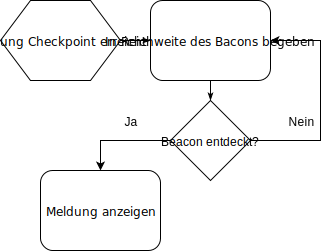
\includegraphics[width=0.5\textwidth]{images/beaconflowchart.pdf}
  \caption{Einsatz eines iBeacons als Flussdiagramm}
  \label{fig:Beaconflowchart}
\end{figure}

Der iBeaconService stellt die Funktionen zum \glqq Hören\grqq auf iBeacons bereit. Zuerst wird ein Delegat \cite{Schatten2010} für den nativen LocationManager erzeugt. Im Anschluss wird sich bei den benötigten EventListenern des Delegaten registriert. Die EventListener sind als Observeables ausgeführt, somit ist es einfach Zustandsänderungen zu detektieren. Listing \ref{lst:ExitRegion} zeigt eine solche Registrierung und die im Erfolgsfall (also hier das Verlassen einer Region) auszuführenden Funktionsaufrufe.

\begin{lstlisting}[float, language=JavaScript, caption= Registrieren beim didExitRegion-EventListener  , label=lst:ExitRegion]
delegate.didExitRegion()
      .subscribe(
      (data) =>{
          this.notificationService.updateWaypoint(data.region.identifier);
        console.log('Gebiet verlassen: ', data.region.identifier);}      
      );
\end{lstlisting}

Die zu entdeckenden Regionen müssen mitgeteilt werden. Dazu verwendet man eine Methode der lokalen Instanz des Plugins. Diese Methode \textit{startMonitoringForRegion(beacon : BeaconRegion)} ist als Promise ausgeführt, da sie asynchron ist. Es ist möglich, den Erfolgs- oder Fehlerfall abzufragen, so dass es eine Mitteilung gibt, wenn die Region nicht beobachtet werden kann. 

\begin{lstlisting}[float, language=JavaScript, caption= Übergabe einer Region an das iBeacon Objekt.  , label=lst:RegisterRegion]
let beacon1 = this.iBeacon.BeaconRegion('Haltestelle 1' , this.rtm.UUID, 10001, 10002);
.
.
.
this.iBeacon.startMonitoringForRegion(beacon1)
       .then(
         (data) => console.log('Native layer received the request to monitoring' + JSON.stringify(data)),
         error => console.error('Native layer failed to begin monitoring: ', JSON.stringify(error))
       );
\end{lstlisting}

  
\section{Local Notification Service}
\label{srv:LNotificationService}
Der Local Notification Service dient dazu Statusinformationen über die jeweiligen Checkpoints als Mitteilung auf dem Bildschirm oder im Notificationcenter eines Smartphone anzuzeigen.
\subsection{Verwendete Plugins}
@ionic-native/local-notification \cite{LocalNotificationPluginDoku}
\subsection{Arbeitsweise}
 Die Nachricht enthält die Uhrzeit und den Checkpoint sowie den Status erreicht bzw. verlassen. Abbildung \ref{fig:Notification} zeigt eine solche Notification.
 
\begin{figure}[htbp] 
  \centering
     \includegraphics[width=0.5\textwidth]{images/Notification.png}
	   \caption{Benachrichtigung im Notification Center}
  \label{fig:Notification}
\end{figure}

Das Erzeugen einer Notification ist in Listing \ref{lst:ScheudleNotification} dargestellt. Basierend auf dem Namen des iBeacons wird die Nachricht generiert. Die \emph{.schedule()}-Methode lässt die Nachricht im Notification Center des Telefons erscheinen.

\begin{lstlisting}[float, language=JavaScript, caption= Erzeugen einer Notification bei Erreichen einer Haltestelle , label=lst:ScheudleNotification]
sendWaypointNotification(identifier: string ){
    let text: string = '';
    text = this.rtm.timeHelper(); switch(identifier){
      case 'Haltestelle 1':{ text = text + ' Haltestelle 1 erreicht.';
                              this.rtm.LOGARRAY.push(text);
                              break;}
      case 'Haltestelle 2':{ text = text + ' Haltestelle 2 erreicht.';
                              this.rtm.LOGARRAY.push(text);
                              break;}
      case 'Haltestelle 3':{ text = text + ' Haltestelle 3 erreicht.';
                              this.rtm.LOGARRAY.push(text);
                              break; }
      default: {text = 'Ein Beacon wurde nicht zugeordnet.'};

    }

    this.notification.schedule({id: 1, title:'BusTracker', text: text, led:'#FF0000'});
  }
\end{lstlisting}

Listing \ref{lst:UpdateNotification} zeigt den Aktualisierungsprozess der Notification. Basierend auf dem Beaconnamen wird die Notification aktualisiert.

\begin{lstlisting}[float, language=JavaScript, caption= Update einer Notification bei Verlassen einer Haltestelle , label=lst:UpdateNotification]
updateWaypoint(identifier : string){
    let text: string = '';
    text = this.rtm.timeHelper();
    switch(identifier){
      case 'Haltestelle 1':{ text =  text + ' Haltestelle 1 verlassen.';
                              this.rtm.LOGARRAY.push(text);
                              break;}
      case 'Haltestelle 2':{ text =  text + ' Haltestelle 2 verlassen.';
                              this.rtm.LOGARRAY.push(text);
                              break;}
      case 'Haltestelle 3':{ text =  text + ' Haltestelle 3 verlassen.';
                              this.rtm.LOGARRAY.push(text);
                              break;}
 		 default: {text = 'Update, kein gueltiger case' };
    }
    this.notification.update({id: 1, text: text, led:'#FF0000'});
  }
\end{lstlisting}



\section{LoadService}
\label{srv:LoadService}
Der LoadService dient zum Laden gespeicherter Werte vom Festspeicher des Telefons in den Laufzeitspeicher \nameref{srv:RTMService}.
\subsection{Verwendete Plugins}
keine 
\subsection{Arbeitsweise}
Die Methoden des LoadService rufen Methoden des \nameref{srv:PersistenzService} auf. Die Rückgabewerte des LoadService sind als Promises ausgeführt, da die Festspeicherzugriffe asynchron erfolgen. 

Listing \ref{lst:LoadUserID} dient als Beispiel und zeigt die Methode um die UserID zu laden. Sie ruft eine Methode des \nameref{srv:PersistenzService} auf, wartet auf das Ergebnis und gibt dieses dann zurück.
  
\begin{lstlisting}[float, language=JavaScript, caption= Laden der UserID , label=lst:LoadUserID]
loadUserID(): Promise<number>{
    console.log('LoadService: LoadUSERID');
    return this.persist.loadUserID();
  }
  \end{lstlisting}
  
\section{SaveService}
\label{srv:SaveService}
Der SaveService hat die Aufgabe, Daten und Werte aus dem Laufzeitspeicher \nameref{srv:RTMService} in den Festspeicher \nameref{srv:PersistenzService} zu überführen.
\subsection{Verwendete Plugins}
keine
\subsection{Arbeitsweise}
Es wird eine im PersistenzSerivce \ref{srv:PersistenzService} vorhandene generische Speichermethode mit Übergabeparametern aufgerufen. Listing \ref{lst:SaveUserID} zeigt den Aufruf. Die Methode des \ref{srv:PersistenzService} ist generisch, so müssen als Argumente ein Label vom Typ String und ein Parameter, hier vom Typ number übergeben werden.

\begin{lstlisting}[float, language=JavaScript, caption= Speichern der UserID , label=lst:SaveUserID]
saveUserID(uid: number){
    console.log('SaveService: UserID');
    this.persistenzService.saveSingleParameter('USERID', uid);
  }
\end{lstlisting}

\section{PersistenzService}
\label{srv:PersistenzService}
Der PersistenzService verwaltet den Festspeicher des Geräts und bietet dafür Lade- und Speichermethoden an.
\subsection{Verwendete Plugins}
@ionic-native/native-storage \cite{NativeStoragePluginDoku}
\subsection{Arbeitsweise}
Der Speicher wird \glqq Native Storage \grqq genannt. Es wird der native Speicher des jeweiligen Geräts verwendet. Das Speichern erfolgt via Key und Value. Soll nun ein Wert geladen werden, so wird die entsprechende \textit{Load}-Methode mit dem Key aufgerufen. Im Beispiel \ref{lst:LoadUserIDPersist} wird die UserID vom Festpeicher geladen. Der Zugriff erfolgt asynchron. Die UserID wird als Promise zurückgegeben.

\begin{lstlisting}[float, language=JavaScript, caption= Laden der UserID vom Native Storage, label=lst:LoadUserIDPersist]
loadUserID(): Promise<number> {
    console.log('PersistenzService: LoadUserID');
    return this.nstorage.getItem('USERID');
  }
\end{lstlisting}

Soll ein Wert gespeichert werden, so kommt die generische Speichermethode zum Einsatz. Hier wird schon wie im \nameref{srv:SaveService} Referenz und Wert übergeben. Die Methode \emph{setItem} ist als
Promise ausgeführt, um der Asynchronität Rechnung zu tragen. 

\begin{lstlisting}[float, language=JavaScript, caption=Generische Speichermethode für Native Storage, label=lst:SaveGeneric]
saveSingleParameter(ref:string, value:any) {
    console.log('PersistenzService: save');
    this.nstorage.setItem(ref, value).then(() =>
      console.log(ref + 'gespeichert!'), (err) => {
      console.log('Fehler beim Speichern von ' + ref + '' + JSON.stringify(err));
    })
  }
\end{lstlisting}

\section{RTMService}
\label{srv:RTMService}
Der Laufzeitspeicher enthält die Daten und Werte, die zur Laufzeit benötigt werden.
\subsection{Verwendete Plugins}
@ionic-native/native-geocoder \cite{GeocoderPluginDoku}
\subsection{Arbeitsweise}
Der RTMService nimmt Werte von verschiedenen  Services entgegen und stellt sie anderen Services zur Verfügung. Alle Dienste die Daten anliefern oder benötigen, instanzieren den RTMService. Die Services, die Speicher- oder Lademethoden benötigen, rufen diese ebenfalls über den RTMService auf.  

\begin{lstlisting}[float, language=JavaScript, caption=Methode zum Persistieren des Appzustandes beim Beenden, label=lst:saveAll]
save(){
    console.log('RTM SaveMethode aufgerufen.')
    this.saveService.saveTrackingIndicator(this.trackingIndicator);
    this.saveService.saveURL(this.URL);
    this.saveService.saveLat(this.lat);
    this.saveService.saveLong(this.long);
    this.saveService.saveADDRESS(this.address);
    this.saveService.saveTrackMarkers(this.trackMarkers);
    this.saveService.saveUserID(this.USER_ID);
    this.saveService.saveTrackingCode(this.trackingCode);
    this.saveService.saveLOGARRAY(this.LOGARRAY);
    this.saveService.saveTrackingID(this.trackingID);
    this.saveService.saveUUID(this.UUID);
  }
\end{lstlisting}


\section{MapsService}
\label{MapsService}
Der MapsService dient zur Darstellung der Eigen- und Fremdposition auf einer Karte. Hier wird auch der zurückgelegte Weg des Beobachteten angezeigt.
 
\subsection{Verwendete Plugins}
@ionic-native/google-maps \cite{GoogleMapsPluginDoku}
\subsection{Arbeitsweise}
Der MapsService bietet unter Verwendung der GoogleMaps \gls{gls:API} die Möglichkeit Dinge auf einer Karte darstellen zu lassen.
Der MapsService erzeugt eine Karte, die zuvor durch Optionen parametriert wird. In Listing \ref{lst:GoogleMapConfig} ist die Instantiierung der Karte dargestellt.

\begin{lstlisting}[float, language=JavaScript, caption= Instantiierung GoogleMap, label=lst:GoogleMapConfig]
this._map = GoogleMaps.create('map_canvas', {
 camera: {
   target: {
     lat: 49.26204150113853,
     lng: 7.36005587579744
   },
  zoom: 15,
  tilt: 30
  }
});
\end{lstlisting}

Die hier angegebenen Optionen sind \emph{map\_canvas}, der Name des <div> in dem die Karte erscheinen soll, und die Position der Kamera. Die Kameraposition wird hier als \emph{target} bezeichnet und enthält einen Längen- sowie einen Breitengrad als Koordinate. Weitere Kameraoptionen sind \emph{zoom}, die Größe des sichtbaren Ausschnitts und \emph{tilt} die Neigung. 

Nachdem die Karte geladen wurde, wird mittels der \emph{.one}-Methode einmalig auf ein Event gewartet. In dieser Situation wird auf das \textbf{MAP\_READY}-Event gewartet. Die \emph{.one}-Methode ist als Promise ausgeführt. Wenn die Karte bereit ist, wird das \emph{mapReady}-Flag auf true gesetzt und die eigene Position abgefragt. Basierend auf den Positionsdaten wird mit \glqq \emph{return this.\_map.addMarker() .. }\grqq{}
eine Markierung auf die Karte gesetzt. Diese Markierung muss ebenfalls parametriert werden. 

Die Optionen sind: 
\begin{description}
\item \textbf{title} Titel bzw. Name des Markers.
\item \textbf{snippet} Zusatztext, der nach dem Klicken auf den Marker angezeigt wird.
\item \textbf{position} Position des Markers als LatLong-Koordinate.
\item \textbf{animation} Animation, mit der der Marker an der in \emph{position} angegebenen Stelle auftaucht.
\end{description}

Der dazugehörige Programmcode befindet sich in Listing \ref{lst:GoogleMapPosition}.


\begin{lstlisting}[float, language=JavaScript, caption=Automatische Darstellung der eigenen Position, label=lst:GoogleMapPosition]
this._map.one(GoogleMapsEvent.MAP_READY).then(() => {
this._mapReady = true;
this._map.getMyLocation().then((location: MyLocation) =>{
return this._map.addMarker({
title: 'Sie sind hier!',
snippet: 'Ihre aktuelle Position',
position: location.latLng,
animation: GoogleMapsAnimation.BOUNCE
})})
});
}
\end{lstlisting}

\section{TrackerService}
\label{srv:TrackerService}

Der Location Tracker stellt die aktuelle \gls{gls:gps} Position des Telefons bereit und überträgt diese an den \nameref{srv:RTMService}. 
Das Ermitteln der \gls{gls:gps} Position ist nicht immer gleich, es wird unterschieden ob sich die Anwendung im Vorder- oder Hintergrund befindet.
\subsection{Verwendete Plugins}
@ionic-native/BackgroundGeolocation \cite{bGeolocation}

@ionic-native/Geolocation \cite{Geolocation}
\subsection{Arbeitsweise}
Sobald der Nutzer auf der Homepage \textbf{Tracking} auswählt, wird die Positionserfassung mittels \textit{startTracking()} gestartet. Nachdem eine Positionsfeststellung erfolgt ist, wird die Position mithilfe des \nameref{srv:APIService} an die \gls{gls:API} weitergegeben. 

Beim Aufruf der Seite wird der  \nameref{srv:iBeaconService} mittels der Methode \textbf{initBeacon()} aktiviert und iBeacons werden nun erkannt.
 
\subsubsection*{Hintergrund}

Wird \emph{Bustracker} in den Hintergrund geschickt, ist das Hintergrundtracking aktiv. Dies geschieht regelmäßig bei der Nutzung einer anderen App oder beim Deaktivieren des Bildschirms. 
Das backgroundGeolocation-Plugin benötigt eine Konfiguration. Diese wird im Code direkt vor dem Aufruf der eigentlichen Methode erzeugt.
\begin{lstlisting}[float, language=JavaScript, caption= Konfiguration Backgroundtracking, label=lst:BTConf]
 let config = {
            desiredAccuracy: 0,
            stationaryRadius: 20,
            distanceFilter: 10,
            debug: false,
            interval: 1000,
            startForeground: false
            stopOnTerminate: true,
        };
\end{lstlisting}

Diese Konfiguration wird an die \emph{.configure()} Methode übergeben, diese liefert ein Observeable vom Typ \emph{BackgroundGeolocationResponse} zurück. 

Das Backgroundtracking wird mittels der \emph{.configure()} Methode konfiguriert und muss explizit durch die \emph{.start()} Methode aktiviert werden. Die \emph{.start()} Methode gibt ein Promise zurück, ob das Starten geglückt ist. Im Erfolgsfall, kann mit \emph{.then(()=>{})} weiterer Code ausgeführt werden, der auf den erfolgreichen Start wartet. Der Fehlerfall kann mittels \emph{.catch((err)=>{})} abgefangen werden. 

Die BackgroundGeolocationResponse wird im angegebenen Intervall (Millisekunden) aktualisiert. Bei \emph{Bustracker} werden aktuell Längen- und Breitengrad als Datum im Latlong- Format verwendet. Diese können vom \emph{location}-Objekt mittels Punktoperator gewonnen werden. Die Verwendung wird in Listing \ref{lst:BTAufruf} gezeigt. Jede Aktualisierung stellt einen Erfolgsfall dar. Ebenfalls im Listing \ref{lst:BTAufruf} zu sehen ist der Code, der im Erfolgsfall ausgeführt wird. Um eine ChangeDetection zu garantieren, wird dieser Code in einer Kopie der aktuellen Angular Zone ausgeführt. Weiterhin werden Längen- und Breitengrad in die entsprechenden Variablen des Laufzeitspeichers \ref{srv:RTMService} geschrieben. 

Die Variable \textbf{bodydata} wird aus aktuellen Daten erzeugt und bei jedem neuen \glqq Fix\grqq an die Methode \emph{postData()} des \gls{gls:API}-Service \ref{srv:APIService} Parameter übergeben. Dies sorgt dafür, dass jede Position an den Server gesendet wird. Im Anschluss wird die neue Position dazu verwendet um eine \glqq menschenlesbare \grqq Adresse zu erzeugen. Diese wird auf Tracking- und WatchPage angezeigt.

  \begin{lstlisting}[float, language=JavaScript, caption= Aktivierung Backgroundtracking, label=lst:BTAufruf] 
 this.backgroundGeolocation.configure(config).subscribe((location) => {

      console.log('BackgroundGeolocation:  ' + location.latitude + ',' + location.longitude);
      
      this.zone.run(() => {
        this.lat = location.latitude;
        this.rtm.lat = location.latitude;
        let bodydata = {id:0, lat: this.rtm.lat, lon: this.rtm.long, time: Date.now(), user_id: this.rtm.USER_ID, beacon_id: 0, beacon_active: true};
        this.apiCall.postData(bodydata);
        console.log('LAT BGTR: '+this.lat);
        this.lng = location.longitude;
        this.rtm.long = location.longitude;
        console.log(' LNG BGTR: '+ this.lng)
        this.geoCode();
      });
      if(this.platform.is('ios'))
      {
        this.backgroundGeolocation.finish().then(
          ()=> console.log('location-tracker.service:backgroundGeolocation.configure: ios finish = ok')); 
      }
    }, (err) => {

      console.log(err);

    });
\end{lstlisting}
Die iOS Plattform benötigt noch eine Mitteilung über das Ende des Backgroundtracking, siehe Listing \ref{lst:finish}.
\begin{lstlisting}[float, language= JavaScript, caption= finish()-Methode für iOS, label=lst:finish]
if(this.platform.is('ios'))
            {
            this.backgroundGeolocation.finish().then(()=> 
            console.log('(...)ios finish = ok'));
            }
\end{lstlisting}


\subsubsection*{Vordergrund}
Sollte sich \emph{Bustracker} im Vordergrund befinden, wird Foregroundtracking benötigt. Analog zum Backgroundtracking wird eine Konfigurationsvariable verwendet, siehe Listing \ref{lst:ForegConf}. 
\begin{lstlisting}[float, language=JavaScript, caption= Konfiguration Foregroundtracking, label=lst:ForegConf]
let options = {
            frequency: 1000,
            enableHighAccuracy: true
        };
\end{lstlisting}

Die Optionen werden beim Aufruf der \emph{watchPosition} Methode übergeben. Die Ausgabe wird mittels \emph{filter((p: any) => p.code === undefined)} so eingestellt, dass nur gültige Werte ausgegeben werden, siehe Listing \ref{lst:watch}.

\begin{lstlisting}[float, language= JavaScript, caption= .watch()-Methode, label=lst:watch]
        this.watch = this.geolocation.watchPosition(options).filter((p: any) => p.code === undefined)
            .subscribe((position: Geoposition) => {
// Run update inside of Angular's zone
                this.zone.run(() => {
                   this.lat = position.coords.latitude;
          this.rtm.lat = position.coords.latitude;
          console.log('FOREGRNDLAT: '+ this.lat);
          this.lng = position.coords.longitude;
          this.rtm.long = position.coords.longitude;
          console.log(' FOREGRNDLONG:'+ this.lng);
          this.geoCode();
                });

            });
\end{lstlisting}

Beim Betreten der \nameref{pag:TrackingPage} wird der \emph{trackingIndicator} abgefragt. Basierend auf dem Wert (true oder false) wird das Tracking mittels \emph{.startTracking()} aktiviert. Es existiert eine \emph{.stopTracking()} Methode, diese beendet das Backgroundtracking und beendet die \emph{subscripton} auf der \emph{.watchPosition()} Methode. Diese Methode wird aber nur benötigt, sollte das Tracking zur Laufzeit beendet werden. Beim Beenden von \emph{Bustracker} wird das Tracking automatisch beendet. Dieses Feature ist in der aktuellen Version des \emph{backgroundGeolocation}-Plugins eingeführt worden. In der Vergangenheit musste die \emph{.stopTracking()}-Methode beim Beenden der App zwingend ausgeführt werden. Listing \ref{lst:stoptrack} zeigt die \emph{.stopTracking()}-Methode.

\begin{lstlisting}[float, language= JavaScript, caption= .stopTracking()-Methode, label=lst:stoptrack]
stopTracking() {
        		console.log('location-tracker.service.stopTracking');
        		this.backgroundGeolocation.stop();
        		console.log('location-tracker.service.stopped by function call stopTracking()');
        		this.watch.unsubscribe('location-tracking.unsubscribed');
    			}	
\end{lstlisting}

\subsection{URLService}
\label{URLService}
Der URLService wird zum Zeitpunkt der Erstellung dieser Arbeit nicht genutzt.
\subsection{Verwendete Plugins}
keine
\subsection{Arbeitsweise}
In der Struktur ist der URLService vorgesehen, um in Zukunft dynamisch URLs für \gls{gls:API}-Zugriffe zu erzeugen. 

	% !TeX root = Bachelorarbeit.tex
\chapter{Fazit und R\'{e}sum\'{e}}
\label{Fazit und R\'{e}sum\'{e}}

Die Fallstudie \emph{Bustracker} wurde mit folgendem Ziel begonnen: \glqq \emph{Mit Hilfe von mobilen Geräten realisieren wir eine Tracking-Möglichkeit für Kinder, die durch einen Bustransport in ländlichen Regionen auf dem Weg zum oder vom Kindergarten, Grundschule oder auch weiterführende Schule befinden.}\grqq{}

Zu diesem Zwecke wurde eine plattformübergreifend lauffähige Applikation für Mobilgeräte vollständig neu entwickelt. Zur Positionsbestimmung werden \gls{gls:gps} und iBeacons verwendet. Die Applikation, ausgeführt als Single Page Application, zeigt die Machbarkeit und kann in Zukunft unter realen Bedingungen getestet werden. 
 
\emph{Bustracker} existiert als Prototyp. Es ist nun möglich, ein Kind auf seinem Weg zur oder von der Betreuung zu beobachten. Die Kombination aus \gls{gls:gps} und iBeacons hat sich als zweckmäßig und vorteilhaft erwiesen. 


\section{Lessons learned}
\label{Lessons learned}

In diesem Abschnitt werden die  im Laufe der Entwicklung aufgetretenen Probleme sowie deren Lösungen diskutiert.  

\subsection{Marker eignen sich nicht zum Anzeigen von Wegen}
Zu Beginn der Entwicklung wurde der Ansatz verfolgt, einzelne Marker in Reihe anzuordnen und so den Fahrweg nachzuvollziehen. Mit Hilfe der \emph{makeTrack(LatLng)}-Methode wurde bei jeder neuen Positionsbestimmung ein Marker auf der Map erzeugt (Listing \ref{lst:makeTrack}). Einige wenige Marker lassen sich ohne Performanceverlust beim scrollen darstellen. Steigt die Zahl der Marker jedoch an, so kommt es zu einer ruckelnden Darstellung. Die Performance der Karte beim Scrollen innerhalb und außerhalb der Karte nahm stark ab, bis hin zur Unzumutbarkeit für den Nutzer.

\begin{lstlisting}[float, language= JavaScript, caption= Erstellen einzelner Marker, label=lst:makeTrack]
  makeTrack(latlong:LatLng){
    let moptions= {
    title:'Strecke',
   snippet: 'Hier faehrt der Bus!',
   position: latlong,
   animation: GoogleMapsAnimation.BOUNCE
  } 
\end{lstlisting}

Als erste Gegenmaßnahme wurde die Darstellung der Marker analog zum Gameloop Konzept verwendet. In ihrer Veröffentlichung  \emph{\textbf{Real Time Game Loop Models for Single-Player Computer Games}} \cite{valente2005real} schreiben die Autoren in Kapitel 2.1, dass die einfachste Game Loop aus den Schritten \glqq User Input\grqq{}, dem\glqq Update\grqq{} und dem \glqq Rendern\grqq{} besteht. In \emph{Bustracker} wäre der User Input die neue Position, das Update wäre das aktualisierte Array und das Rendern der Aufruf einer Methode zum Darstellen einer Gruppe von Markern, eines sogenannten Clusters.
Eine Testimplementierung zeigte bereits zu Beginn, dass hierdurch kein Performancegewinn zu erzielen ist.  

Als Lösung wurde der Weg über die Polyline gewählt. Die Polyline ist eine Linie, welche die sie definierenden Punkte verbindet. Das Zeichen einer Linie beansprucht wesentlich weniger Ressourcen als das Zeichnen einer Grafik in Form eines Markers für jeden einzelnen Punkt. Listing \ref{lst:polyline} zeigt die Verwendung der Polyline.
\vspace{12px}
\begin{lstlisting}[language= JavaScript, caption= Zeichnen einer Polyline auf einer Google Map, label=lst:polyline]
makePolyFromArray(array: any[]){
this._map.addPolyline({
points: array,
'color' : '#AA00FF',
'width': 10,
'geodesic': true
});}
\end{lstlisting}
Die Punkte werden als Array vom Typ LatLng[] übegeben. 

Weitere Parameter sind: 
\begin{itemize}
\item[\textbf{color}]
Farbe der Linie in Hexadezimalschreibweise
\item[\textbf{width}]
Breite der Linie in Pixel
\item[\textbf{geodesic}]
Falls true gewählt ist, passt sich die Linie der Erdkrümmung an.
\end{itemize}

\subsection{Polyline wurde nicht gezeichnet, maximal 100 Punkte sind erlaubt}
Um den zurückgelegten Pfad vom beobachteten Nutzer an den Straßenverlauf anzupassen, wird die Google Maps Roads API \cite{RoadsAPIDoc} verwendet. Diese nimmt eine Menge von LatLong Koordinaten entgegen und interpoliert, wenn gewählt, die Strecke mit zusätzlichen Punkten. Diese Punkte werden im \gls{gls:json}-Format zurückgegeben und können zur Darstellung einer Linie auf der Karte verwendet werden.

\begin{lstlisting}[float, language= JavaScript, caption= Verwendung der RoadsAPI durch \emph{Bustracker}, label=lst:MapsApi]
snapToRoad(dinger: LatLng[]): Promise<LatLng[]> { 
  console.log('Hello SnapToRoad');
  let prom = new Promise<LatLng[]>((resolve, reject) => {
  let payload: string = '';
  let ret: LatLng[] = [];
  for (let i: number = 1; i <= 100; i++) {
    payload = payload + dinger[i].lat + ',' + dinger[i].lng;
    if (i < 100)
    payload = payload + '\|';
  }
    this.http.get('https://roads.googleapis.com/v1/snapToRoads?path=' + payload
    + '&interpolate=true&key=<Der API-Key>').subscribe((data) => {
    data['snappedPoints'].forEach((itr) => {
    ret.push(new LatLng(itr.location.latitude, itr.location.longitude));
  });
      resolve(ret);
    }), (err) => {
        reject('Fehler beim SnapToRoad' + JSON.stringify(err));
      };
   });
    console.log('Bye SnapToRoad');
    return prom;
  }
}
\end{lstlisting}

Listing \ref{lst:MapsApi} zeigt die Methode, die eine Menge von LatLong-Koordianten an die Google Maps Roads \gls{gls:API} übergibt und die Antwort in Form eines Promise zurückgibt. Die ersten Versuche, die Koordinaten aus der \emph{Bustracker}-\gls{gls:API} zu verwenden, führten nicht zum Erfolg. Nach Einfügen von Konsolenausgaben und teilweisem Auskommentieren von Code wurde ersichtlich, dass der Fehler im Bereich des GET-Requests lag. Um das \glqq err \grqq{} Objekt auf der Konsole lesbar auszugeben, wird es mit Hilfe der \emph{JSON.stringify()}-Methode in einen String umgewandelt. Aus der Fehlermeldung ging hervor, dass die Anzahl der an die Google Maps Road \gls{gls:API} übergebenen Punkte zu hoch ist, maximal 100 sind erlaubt. Um diesem Umstand Rechnung zu tragen wurden die Zeilen 6 -10 aus dem Listing \ref{lst:MapsApi} eingefügt. Diese Schleife sorgt nun dafür, dass nur die letzten 100 Elemente an die Google Maps \gls{gls:API} geschickt werden. Die Strecke wird sukzessive in Abschnitten gezeichnet.

\subsection{API-KEY für native Android und iOS Anwendungen}
Bei der Installation des Google Maps Plugins \cite{GoogleMapsPluginDoku} muss im Konsolenbefehl (Listing \ref{lst:mapsPlugin}) der API-Key für die jeweilige Plattform angegeben werden.



\begin{lstlisting}[float,language= Bash, caption= CLI Befehle - Installation Google Maps Plugin , label=lst:mapsPlugin]
$ ionic cordova plugin add cordova-plugin-googlemaps --variable API_KEY_FOR_ANDROID="YOUR_ANDROID_API_KEY_IS_HERE" --variable API_KEY_FOR_IOS="YOUR_IOS_API_KEY_IS_HERE"
$ npm install --save @ionic-native/google-maps
\end{lstlisting}

Dieser Key ist über die Google Developer Konsole \cite{GoogleDevConsole} einzurichten und zu beziehen. Googles  Dokumentation zu Maps enthält eine ausführliche Anleitung zum Erzeugen von Keys. \cite{GoogleGetKey}.


\section{Ausblick}
\label{sec:Ausblick}
Die Anwendung wird kontinuierlich weiterentwickelt und neue Features werden implementiert. An dieser Stelle wird ein Überblick über weitere Entwicklungsmöglichkeiten von \emph{Bustracker} gegeben.

\subsection[Freies Kartenmaterial]{Umstellung auf freies Kartenmaterial}
Um in Zukunft weniger abhängig von Google und deren \glspl{gls:API} zu sein, soll die Anwendung auf freies Kartenmaterial umgestellt werden. Das Kartenmaterial soll von \gls{gls:OSM} bezogen werden \cite{OSM}. Das Anpassen an den Straßenverlauf soll mittels der \gls{gls:OSRM} \cite{OSRM} durchgeführt werden. 

\subsection[Ankunftszeitberechnung]{Berechung der Ankuftszeit am Ziel}
Ein geplantes Feature ist die Berechnung der Ankunftszeit an einem Ziel. Dem Beobachter soll mitgeteilt werden, zu welcher Zeit die Ankunft am Ziel erwartet wird. Zunächst soll dies mit Hilfe der Google Distance \gls{gls:API} gelöst werden. In einer späteren Iteration soll dies ebenfalls unter Verwendung der \gls{gls:OSRM} durchgeführt werden. 

\subsection{Nutzerauthentifizierung}
Zukünftig soll eine Authentifizierung durchgeführt werden, um nur befugte Beobachter für ein bestimmtes Gerät zuzulassen.
Verschiedene Lösungen sind denkbar, z. B. das Generieren eines einzigartigen Schlüssels für jeden einzelnen Trackingvorgang. 
Denkbar ist auch eine Konfiguration einer Art Familie, in der einzelne Geräte einem Beobachter zugewiesen werden können.

\subsection{Sparchassistentenunterstützung}
Es wäre denkbar, die Datenbankeinträge des Servers mittels sogenannter Skills für Sprachassistenten abzurufen. Die rein auditive Darstellung könnte die momentane geocodierte Position bzw. den jeweiligen Checkpoint enthalten. 

\section{Fazit}
\label{Fazit}

\emph{Bustracker} ist ein Beispiel für eine Anwendung im Rahmen der Digitalisierung des ländlichen Raumes. Zurzeit ist die Anwendung im Status eines Prototyps. Durch kontinuierliche Weiterentwicklung, vor allem das Einarbeiten der im Ausblick genannten Features und Anpassungen an zukünftig evaluierten Nutzungsszenarien, wird \emph{Bustracker} zu einer höheren Sicherheit auf dem Schulweg beitragen.
	

	%\input{anhang}
	
	\singlespacing
	\bibliographystyle{unsrtdin}
	\bibliography{literatur}
	\nocite{*} % nicht referenzierte Literatur anzeigen
	\addcontentsline{toc}{chapter}{Literatur}
	

\raggedright

\todos

\end{document}
